\subsection{Architecture de communication hybride \og orientée 
événements\fg{}}
\label{sec:comm_event}

Cette architecture est une combinaison des contributions présentées dans 
\cite{Desprat2016,Desprat2017}. Contrairement à l'architecture précédemment 
décrite, celle-ci repose sur le paradigme événementiel et fonctionne en accord 
avec le framework orienté événements présenté dans la Section 
\ref{sec:modele_event}. Trois aspects de l'architecture de communication hybride 
orientée événements sont mis en valeurs dans cette thèse : la présentation des 
composants de l'architecture \gls{P2P} peu couplé, un système de gestion de 
cohérence ainsi qu'un protocole de 
synchronisation utilisant un journal d'événements partagé entre les pairs.
 
\begin{figure}[ht]
	\centering
	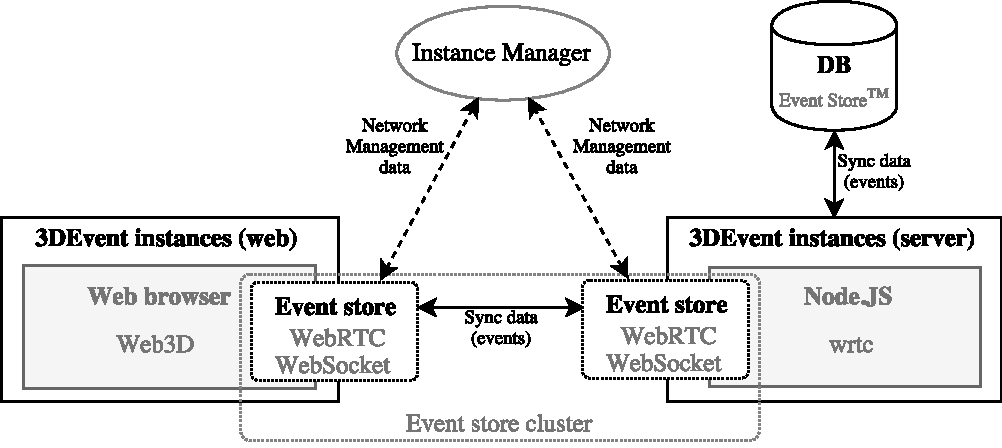
\includegraphics[width=\columnwidth]{eps/archi.pdf}
	\caption{Architecture de communication \og orientée événements\fg{}}
	\label{fig:archievent}
\end{figure}

\subsubsection{Spécificité des composants de l'architecture}
L'Event Store est un composant clé dans le traitement des événements. Présent 
sur chaque pair, il prend en entrée des événements de deux natures : ceux qu'il a 
générés via la partie commande (internes) et ceux reçus via le réseau 
principalement (externes). 
L'Event Store produit en sortie des événements dits \og 
cohérents\fg{} qui peuvent être publiés par la suite sur l'Event Publisher.
Un Event Store est composé de deux types d'éléments : 
\begin{itemize}
	\item l'\gls{ESM} qui gère les flux d'événements : structure de données 
	présente dans chaque Event Store qui doit permettre l'accès en lecture et en 
	écriture des agrégats qu'elle contient. 
	Un \gls{ESM} contient des flux d'événements ordonnés temporellement 
	pour chaque agrégat géré ;
	\item les \glspl{NB} qui servent de connecteurs réseaux : responsables de la 
	gestion d'une connexion \gls{P2P}, i.e. gère le flux de données entrant et 
	sortant vers chaque pair auquel ils sont reliés.
\end{itemize}

La Figure \ref{fig:archievent} montre des pairs (appelés instances) de différentes 
natures :
\begin{itemize}
	\item Instance Web :  produit, stocke et relaie des événements aux autres 
	instances.
	\item Instance Serveur : stocke et relaie des événements aux autres instances 
	et à la base de données. 
\end{itemize}

En plus de servir de relais comme une Instance Serveur, une Instance Web est 
productrice d'événements. C'est en général le type d'instance par lequel un 
utilisateur accédera à l'application. Les Instances Serveurs, en comparaison avec 
l'architecture présentée précédemment, sont des \og serveurs\fg{} qui participent 
directement à la couche réseau. En cela, ils aident à la dissémination des données 
et peuvent rapidement être montés pour garantir une disponibilité des données 
auprès des autres instances (notamment en cas de panne).
Toutes les instances sont coordonnées par l'\gls{IM} qui est responsable de mettre 
les pairs en relation. Il est notamment le serveur responsable dans le mécanisme 
de \textit{signalling}. 
L'ensemble des Event Stores forme une grappe qui gère le 
journal d'événements partagé de manière répartie entre toutes les instances.
\subsubsection{Gestion du stockage}

Lorsque l'Event Store reçoit de nouveaux événements, l'\gls{ESM} crée ou 
récupère le flux d'événements associé à l'agrégat dans un premier temps. Puis, il 
stocke l'événement à la suite de ceux présents dans le flux de l'agrégat sur le pair, 
localement.
Par ailleurs, dans un contexte industriel de collaboration, l'information doit être 
disponible sur le long-terme, facilement accessible par l'entreprise. 
La persistance à long-terme du système stocke le journal d'événements qui est la 
source de vérité de l'application. Elle peut également stocker des projections 
prédéfinies, calculées à la volée ou encore des \textit{snapshots} de l'application.

Sur la base du modèle orienté événements, les données à stocker sont les 
événements. Ils sont immuables et constituent des données purement 
fonctionnelles (Section \ref{sec:es-vs-cs}).
L'utilisation d'une base de données fonctionnelle permet de se reposer sur 
l'immuabilité des événements.
L'argument souvent opposé à l'utilisation de telles bases est le coût de l'espace de 
stockage. Or le coût de la redondance et de la non localité du traitement des 
données, a chuté au cours de ces dernières années. 
Une base de données dont les données muent -- i.e où chaque donnée peut être 
modifiée à n'importe quel moment -- ne permet pas de conserver l'historique des 
modifications (ex : \textit{Active Record}). Dans une base de données dite 
fonctionnelle, les données stockées sont immuables -- i.e. elles ne peuventt être modifiée \textit{a posteriori} et fait seulement référence à 
d'autres données immuables. Une telle base de données est \og \textit{une interface vers 
des \textit{snapshots} versionnés}\fg{} \cite{Meric2012}.

Dans le cas de l'\gls{ES}, les événements sont considérés comme des deltas 
(avec quelques métadonnées supplémentaires) sur les agrégats. C'est donc sous 
leur forme originale qu'ils sont stockés. Cela évite également les transformations 
de données (et la perte d'information ou l'ajout de complexité) qui sont nécessaires 
dans les \glspl{ORM}, en lecture et en écriture.

\subsubsection{Gestion de la synchronisation et de la cohérence}
Dans \cite{Desprat2017} lorsqu'un pair initialise ou rejoint la séquence pour 
rejoindre une session collaborative, il évolue pour se synchroniser et intégrer les 
nouveaux événements à son journal.
La Figure \ref{fig:connexionpairs} représente la séquence d'actions nécessaire à 
une instance 3DEvent ($idA$) pour rejoindre le réseau contenant déjà d'autres 
instances 3DEvent. L'action \textit{join} est exécutée lorsqu'un utilisateur envoie 
ses informations de connexion sur un portail de connexion (à partir d'une instance 
web) ou lorsqu'une instance serveur est lancée. Cette action ajoute le nouveau 
pair à la liste des pairs présents sur le réseau. Cette liste est gérée par le 
gestionnaire d'instance, qui la retourne au pair pour lui indiquer les pairs 
avec lesquels il doit se connecter.
Pour chaque pair $idB$ de la liste retournée $ids$, $idA$ utilise le mécanisme de 
signalisation (offre/demande). Le mécanisme est déclenché par l'instanciation d'un 
\gls{NB} dans l'Event Store de $idA$ puis celui de $idB$. Afin de resynchroniser 
les deux pairs (après cette série d'échanges asynchrones), $idA$ et $idB$ 
s'échangent des méta-données sur la situation respective de leurs \gls{ESM} 
afin de se synchroniser.

\begin{figure}[h]
	\noindent
	\centering
	\includegraphics[width=\columnwidth]{connection.eps}
	\caption{Protocole de connexion au réseau d'instance 3DEvent}
	\label{fig:connexionpairs}
\end{figure}

\paragraph{Cohérence d'un flux d'agrégat}
Les événements sont considérés comme \og cohérents\fg{}  lorsqu'il n'y a pas 
d'erreur de cohérence dans l'agrégat, i.e. lorsqu'il n'y a pas de doublon dans les 
numéros de versions et qu'ils sont bien ordonnés. Lorsqu'un \gls{ESM} ne 
rencontre pas de problème de cohérence, alors le 
dernier index correspond au numéro de version de l'agrégat. 

Lorsque l'Event Store reçoit un événement interne, l'\gls{ESM} récupère (ou crée) 
le flux d'événements associés à l'agrégat référencé par l'événement. 
La cohérence de la version est alors vérifiée en comparant la version attendue 
(exposée dans les méta-données de l'événement) et la version actuelle de 
l'agrégat. 
Si les deux numéros de version sont identiques, l'événement est ajouté à la fin du 
tableau du flux pour être stocké dans l'\gls{ESM}, sinon une exception indiquant 
l'incohérence est levée. 


\paragraph{Mécanisme de gestion de version}
3DEvent intègre une procédure de gestion de version dans l'\gls{EventStore} afin 
de gérer au mieux la cohérence des données. 
Pour être cohérent, le flux de l'agrégat concerné par ces 
événements doit produire une nouvelle version, sans être en conflit avec la 
précédente. En passant la version attendue $v_a$ au gestionnaire de conflits, on 
est à même de la comparer avec la version courante $v_c$. Il existe deux cas de 
conflits~: 
\begin{enumerate}[label=\alph*)]
	\item \label{i:vi} $v_a$ correspond à la valeur d'initialisation du flux : après une 
	action, la version initiale de l'agrégat ne peut être identique ;
	\item \label{i:vdiff} $v_a$ est différente de la version $v_c$ : l'Event Store 
	propage une information incohérente si la version attendue est inexacte.
\end{enumerate}

La cohérence est gérée par l'Event Store à plusieurs niveaux dans le pair :  
localement lors de la génération d'événements par le pair et au niveau du réseau 
\gls{P2P} lors de la réception d'événements.
Les nouvelles données qui entrent dans un pair doivent nécessairement être en 
cohérence avec celle qui sont déjà certifiées cohérentes.

L'algorithme \ref{algo:addevent} permet de détecter une incohérence lors de 
l'arrivée d'un nouvel événement. Cet événement est fourni avec une version qui 
correspond au numéro de version attendu du flux de l'agrégat 
(\textit{stream}) auquel il est rattaché. Si le flux n'existe pas, il est créé, sinon il 
faut vérifier qu'il n'existe pas déjà un événement stocké à la version donnée pour 
pouvoir ajouter l'événement au flux, sinon une exception indiquant un problème de 
cohérence est levée.

\begin{algorithm} % enter the algorithm environment
	\caption{Ajout d'un événement dans l'Event Store} % 
	%give the algorithm a caption
	\label{algo:addevent} % and a label for \ref{} commands later in the document
	\begin{algorithmic} % enter the algorithmic environment
		\Require streamId: string, event: EventStoreEvent, version: number
		\Ensure event
		\State $stream \leftarrow streams.getOrCreate(streamId);$
		\If{$ stream.has(version)$}
		\State $throwExceptionVersion(stream,version)$
		\EndIf
		\State $stream.data.set(version,event) $
	\end{algorithmic}
\end{algorithm}

\subsubsection{Topologie et Protocole d'échange}
L'architecture hybride orientée \og événements\fg{} tire profit de la présence des 
Instances Serveur pour réduire la responsabilité des pairs producteurs (Instances 
Web) dans la distribution des données. En effet, les Instances Serveur qui 
participent au réseau permettent de proposer plus de points de distribution de 
données directement reliés à la base de données. De ce fait, la politique de 
connectivité entre les pairs peut être réduite, le réseau a une topologie 
partiellement maillée (\textit{partial mesh topology}). 

Le protocole d'échange est décrit dans l'annexe \ref{annexe:protocole}. En passant 
de l'instanciation d'une connexion à l'échange de méta-données pour se 
synchroniser, le pair agit comme une machine à état concernant la transmission 
des données. La Figure \ref{fig:connexionpairs} présente une partie des échanges 
liés à ce protocole dans la partie \textit{\gls{P2P} network creation}. Les 
méta-données échangées permettent aux n\oe uds de savoir \og qui possède 
quoi\fg{} sur le réseau pour pouvoir ensuite demander les événements qui leur 
manquent. 


\begin{algorithm} % enter the algorithm environment
	\caption{Synchronisation d'un n\oe ud de l'Event Store partagé} % 
	%give the algorithm a caption
	\label{algo:synchnode} % and a label for \ref{} commands later in the document
	\begin{algorithmic} % enter the algorithmic environment
		\Require $node : ClusterNode$
		\Ensure $nodeState == synchronized$
		\State $nodeMetadata \Leftarrow node.getMetadata()$
		\If{$nodeMetadata != \{\} $}
		\State $streamsToSync \Leftarrow metadata.getDiff(nodeMetadata)$
		\While{$streamsToSync > 0$}
		\State $streamToSync \Leftarrow streamsToSync.pop()$
		\State $events \Leftarrow  node.getEvents(streamToSync)$
		\If{$! streamToSync.has(version)$}
		\For {$event$ \textbf{in} $events$}
		\State $processEvent(event.streamName, event, 
		event.version)$
		\EndFor 
		\EndIf
		\State $streamsToSync \Leftarrow metadata.getDiff(nodeMetadata)$
		\EndWhile
		\EndIf
		\State $node.endSync()$
	\end{algorithmic}
\end{algorithm}

Cette étape de synchronisation d'Event Store entre deux n\oe uds est reprise en 
détail dans l'algorithme \ref{algo:synchnode}. Le n\oe ud courant demande le 
différentiel (\textit{diff}) entre ses flux et ceux du n\oe ud $node$ pour 
connaître quels sont les flux à synchroniser. Si un n\oe ud possède les données 
demandées il les envoie. Si le n\oe ud courant reçoit à nouveau les mêmes 
données, elles sont ignorées par le système.




%\tod{categories: type d’agregat
%	c’est un flux liés a une categorie (exemple geometries) tous les events liés à 
%la 
%	categorie.}
%
%\tod{metadata phase sync permet a un nouveau noeud de recup toutes les info 
%	manquantes et de les demander de maniere repartie a tous les noeuds}
%

\subsubsection{Discussion sur l'architecture de communication \og orientée  
événements\fg{}}

L'architecture de communication orientée événement utilise un intergiciel réactif : 
elle consomme des notifications d'événements et permet le traitement asynchrone 
de messages. Bien que le découplage proposé par ce système offre des 
avantages importants dans un fonctionnement décentralisé, il peut également 
être à l'origine d'incertitudes causées par les 
délais des notifications, notamment lors de l'apparition de conflits.

Tous les pairs qui participent à la gestion de 
données (producteurs et consommateur) sont au même 
niveau dans la couche \gls{P2P}. Cette situation ne propose qu'une flexibilité 
limitée dans le passage à l'échelle et dans la gestion de l'attrition. L'équilibre entre 
les producteurs 
et les consommateurs doit être assez stable pour ne pas surcharger certaines 
parties du réseau. C'est une des raisons pour lesquelles le réseau 
\gls{P2P} est renforcé par la présence de pairs destinés à 
faire le relais dans la distribution des données. 


\paragraph{\glspl{CRDT} basés opérations}
La gestion de la cohérence dans un \gls{SEC} massif est souvent étudiée à 
travers le prisme des \glsreset{CRDT}\glspl{CRDT}. Les \glspl{CRDT} sont des 
types de 
donnés répliqués qui convergent prenant en compte des mises à jours 
concurrentes. 
Un \gls{CRDT} peut être mis à jour sans nécessiter la coordination des répliques. 
Cela rend les \glspl{CRDT} hautement disponibles pour les opérations d'écriture. 
Les \glspl{CRDT} peuvent être classés selon deux catégories : les \glspl{CRDT} 
orientés état (CvRDTs ou \textit{\textbf{convergent} replicated data types}) et les 
\glspl{CRDT} basés opération (CmRDTs ou\textit{ \textbf{commutative} replicated 
data types}). Les \glspl{CRDT} orientés état sont conçus pour disséminer un 
état parmi les répliques alors que les \glspl{CRDT} basés opérations sont conçus 
pour disséminer des opérations.

Les répliques de CmRDT sont garanties de converger si les opérations sont 
disséminées au travers d'un intergiciel à transmission fiable et causale 
(\textit{reliable causal broadcast} (RCB)) et si leurs opérations concurrentes sont 
commutatives.

Les CvRDTs ne nécessitent pas d'intergiciel de messagerie mais une bande 
passante croissante dû à l'augmentation de la taille de l'état. La convergence 
passe par une fonction de fusion définie comme une jointure.

L'exécution d'une opération sur un CmRDT s'effectue en deux phases, 
\textbf{préparation} et \textbf{effet} (aussi appelées \textit{atSource} et 
\textit{downstream} \cite{Shapiro2011}. La production du message représentant 
l'opération se base sur l'opération et éventuellement l'état courant pendant la 
phase de préparation du CmRDT.

\paragraph{Relation entre \glspl{CRDT} et \acrlong{ES}}
Les deux phases de mise à jour d'un CmRDT, \textbf{préparation} et \textbf{effet}, 
sont très proches des phases de mise à jour des entités en \gls{ES}, 
\textbf{traitement de 
la commande }(\textit{command handler}) et \textbf{traitement des événements} 
(\textit{event 
publisher}). 

Durant le \textbf{traitement de la commande}, une commande entrante peut être 
validée en fonction de l'état de l'entité sur lequel elle est appliquée et, si elle l'est, 
un événement représentant l'effet de la commande est inscrit dans le journal 
d'événements. Cela correspond à la phase de préparation d'un CmRDT. 

Durant la 
phase de \textbf{traitement des événements}, l'événement écrit est consommé à 
partir du journal d'événements et utilisé pour mettre à jour l'état courant de l'entité. 
Cela correspond à appliquer la représentation de l'opération produite à l'état du 
CmRDT local durant la phase \textbf{effet}. Le \gls{CQRS} associé à l'\gls{ES} 
distingue ces deux phases et fournit une couche d'abstraction supplémentaire 
permettant à l'application de définir des 
commandes et des traitements d'événements spécifiques au domaine.

Les CmRDTs et les entités issus de l'\gls{ES} doivent pouvoir à la fois 
consommer des événements issues d'autres acteurs et produire des événements 
pour les autres acteurs. Cette collaboration est nécessaire pour déployer plusieurs 
répliques de la même entité. 

La représentation des données 3D dans cette thèse ne permet pas l'utilisation de 
CmRDTs comme dans ChainVoxel \cite{Imae2016}. Cette représentation 
combinée à notre modèle \gls{CQRS} et \gls{ES} pourrait permettre d'améliorer le 
passage à l'échelle et garantir la convergence des répliques de manière formelle.
%
%vers le même état qui peuvent être classé da selon deux catégories
%Les données 3D telles qu'elles sont 
%modélisées ne rentrent pas dans cette catégorie très puissante pour gérer la 
%cohérence. 
%Cependant, le modèle événementiel fournit, avec son approche fonctionnelle, 
%proche des \gls{CRDT} \textit{Grow-only Set} (qui n'autorise que les ajouts),.




